\documentclass[12pt,a4paper]{article}

% Essential packages
\usepackage[utf8]{inputenc}
\usepackage[T1]{fontenc}
\usepackage{amsmath,amssymb,amsthm}
\usepackage{graphicx}
\usepackage{hyperref}
\usepackage{natbib}
\usepackage{algorithm}
\usepackage{algorithmic}
\usepackage{booktabs}
\usepackage{multirow}
\usepackage{geometry}
\usepackage{placeins}
\usepackage{microtype}
\usepackage{tikz}
\usepackage{listings}
\usepackage{xcolor}

% Page geometry
\geometry{margin=1in}
\setlength{\emergencystretch}{2em}

% Theorem environments
\newtheorem{theorem}{Theorem}
\newtheorem{lemma}{Lemma}
\newtheorem{proposition}{Proposition}
\newtheorem{definition}{Definition}

% Custom commands
\newcommand{\E}{\mathbb{E}}
\newcommand{\Var}{\mathrm{Var}}
\newcommand{\Cov}{\mathrm{Cov}}
\newcommand{\N}{\mathcal{N}}
\newcommand{\R}{\mathbb{R}}
\newcommand{\bX}{\mathbf{X}}
\newcommand{\bZ}{\mathbf{Z}}
\newcommand{\by}{\mathbf{y}}
\newcommand{\bU}{\mathbf{u}}
\newcommand{\bbeta}{\boldsymbol{\beta}}
\newcommand{\btheta}{\boldsymbol{\theta}}
\newcommand{\bmu}{\boldsymbol{\mu}}
\newcommand{\bSigma}{\boldsymbol{\Sigma}}

% Code listing style
\lstset{
    basicstyle=\ttfamily\small,
    keywordstyle=\color{blue},
    commentstyle=\color{gray},
    stringstyle=\color{red},
    breaklines=true,
    frame=single,
    language=Python
}

\title{TabMixNN: A Unified Deep Learning Framework for Structural Mixed Effects Modeling on Tabular Data}

\author{
    Deniz Akdemir \\
    \texttt{deniz.akdemir.work@gmail.com}
}

\date{\today}

\begin{document}

\maketitle

\begin{abstract}
In this article we describe TabMixNN, a PyTorch implementation of neural prediction models for grouped tabular data. A formula-based encoder combines a fixed-effect design with variational random effects, followed by a neural backbone and outcome-specific heads. The implementation provides eight selectable random-effect covariance structures and ten outcome families, including discrete and continuous survival outcomes. We describe its noncentered variational objective, the dimensions of its encoder, and the sequential static--dynamic structural block used by the default GSEM implementation. Evaluation distinguishes held-out observations from known groups from prediction for entirely unseen groups. Reproducible experiments over five fixed splits per prediction regime on five regression and five classification datasets compare TabMixNN with classical mixed models, a fixed-effects neural control, XGBoost and Random Forest. This exploratory dataset set contains 180 to 7,584 observations per task and was revised after an earlier evaluation. Benefits depend on the prediction setting: fitted group information improves known-group prediction relative to the fixed neural control, whereas performance for unseen groups is mixed. The classical mixed model has higher five-split mean AUROC than TabMixNN on all five unseen-group classification tasks. Primary-split calibration diagnostics show that the classification probabilities can be too extreme and can underpredict event frequency. A scalar linear Sleepstudy check gives predictions close to an independently fitted ML mixed model. This agreement does not establish REML equivalence. Single-feature ablations provide descriptive sensitivity summaries, and latent variational draws alone are not full posterior predictive uncertainty.

\end{abstract}

\section{Introduction}

Grouped tabular data contain both covariate information shared across observations and information specific to subjects, sites or other grouping units. The prediction task matters: a held-out observation from a known subject can use that subject's fitted effects, whereas an entirely new subject has no observed outcomes from which to estimate them. Classical mixed-effects models provide a principled formulation of these distinctions \citep{bates2014fitting, pinheiro2006mixed}. Their linear, generalized and nonlinear variants have different modeling assumptions; a neural model should not be justified by treating all classical mixed models as linear predictors.

Combining nonlinear prediction with random effects is established work. LMMNN integrates neural networks with a Gaussian mixed-model likelihood \citep{simchoni2023integrating}; GPBoost combines boosting with Gaussian processes and grouped random effects \citep{sigrist2022gaussian}. TabMixNN addresses an implementation question within this literature: how to expose a common formula interface for latent mixed-effects encoding, alternative neural transformations and several outcome likelihoods. Its innovation-coordinate variational approximation and placement of group effects before the nonlinear decoder distinguish the implementation, but do not establish superiority over existing mixed-effects machine-learning methods.

We introduce TabMixNN (Mixed Effects Neural Networks for Tabular Data), a modular implementation integrating:

\begin{itemize}
    \item \textbf{Mixed-effects modeling}: Variational random effects with flexible covariance structures including autoregressive (AR), kinship, and Gaussian process kernels
    \item \textbf{Modern neural architectures}: Generalized Structural Equation Models (GSEM) with static/dynamic structure learning and spatial-temporal manifold networks
    \item \textbf{Diverse outcome families}: Support for ten outcome families covering regression, classification, multivariate, multi-label and survival outcomes
    \item \textbf{Interpretability}: Single-feature ablation values, variance decomposition, and parameter extraction for model understanding
    \item \textbf{Accessible interface}: R-style formula syntax familiar to statisticians
\end{itemize}

The framework is designed to be modular, extensible, and accessible to both statisticians familiar with classical mixed-effects models and machine learning practitioners seeking to incorporate hierarchical structure into deep learning workflows.

\subsection{Contributions}

Our main contributions include:

\begin{enumerate}
    \item A modular architecture that cleanly separates mixed-effects encoding, backbone networks, and outcome-specific heads, enabling flexible composition of components
    \item Variational treatment of random effects with support for eight selectable covariance structures (IID, AR1, ARMA, Compound Symmetry, Unstructured slopes, Kronecker, Kinship, Gaussian Process)
    \item Two complementary backbone architectures: GSEM with ordered triangular structure and gated attention, and Manifold networks for spatial-temporal data
    \item Support for ten implemented outcome families enabling multitask learning across heterogeneous outcome types
    \item Interpretability tools bridging deep learning and classical statistics (parameter extraction, variance components, single-feature ablation values)
    \item An open-source PyTorch implementation with extensive documentation
\end{enumerate}

\subsection{Paper Organization}

The remainder of this paper is organized as follows: Section \ref{sec:background} reviews related work in mixed-effects modeling and deep learning for tabular data. Section \ref{sec:methods} presents the TabMixNN framework in detail, including the mixed-effects encoder, backbone architectures, outcome families, and training procedures. Section \ref{sec:usage} describes the software interface and typical usage patterns. Section \ref{sec:benchmarks} presents empirical benchmarks on diverse datasets. Section \ref{sec:discussion} concludes with discussion and future directions.

\section{Background and Related Work}
\label{sec:background}

\subsection{Classical Mixed-Effects Models}

Linear mixed-effects models (LMMs) extend linear regression to handle grouped or hierarchical data by partitioning variation into fixed effects (population-level parameters) and random effects (group-specific deviations). The canonical LMM formulation is:

\begin{equation}
    \by_i = \bX_i\bbeta + \bZ_i\bU_i + \boldsymbol{\epsilon}_i
\end{equation}

where $\by_i$ is the response vector for group $i$, $\bX_i$ contains fixed-effects covariates, $\bZ_i$ contains random-effects covariates, $\bbeta$ are fixed-effects coefficients, $\bU_i \sim \N(0, \bSigma_u)$ are random effects, and $\boldsymbol{\epsilon}_i \sim \N(0, \sigma^2\mathbf{I})$ is residual error.

Estimation typically proceeds via maximum likelihood (ML) or restricted maximum likelihood (REML) using Expectation-Maximization (EM) or direct optimization. Popular implementations include R's \texttt{lme4} \citep{bates2014fitting} and \texttt{nlme} \citep{pinheiro2006mixed} packages.

Extensions include:
\begin{itemize}
    \item \textbf{Generalized LMMs (GLMMs)}: Allow non-Gaussian outcomes via link functions \citep{mcculloch2001generalized}
    \item \textbf{Nonlinear mixed-effects models (NLMMs)}: Nonlinear mean functions \citep{lindstrom1990nonlinear}
    \item \textbf{Flexible covariance structures}: AR, ARMA, compound symmetry for longitudinal data
    \item \textbf{Spatial models}: Gaussian processes, SPDE for spatial correlation \citep{lindgren2011explicit}
\end{itemize}

Classical mixed models remain relevant comparators. Their suitability depends on the specified mean structure, covariance assumptions and computational scale, rather than on a categorical distinction between statistical models and neural networks.

\subsection{Deep Learning for Tabular Data}

TabNet \citep{arik2021tabnet}, FT-Transformer \citep{gorishniy2021revisiting}, SAINT \citep{somepalli2021saint} and TabPFN \citep{hollmann2023tabpfn} motivate flexible predictors for tabular data. Standard tabular prediction and mixed-effects prediction nevertheless pose different questions about within-group information. LMMNN \citep{simchoni2023integrating} and GPBoost \citep{sigrist2022gaussian} directly address correlated observations. The present experiments compare TabMixNN with a fixed neural control, classical mixed models and conventional tree methods. They do not compare against LMMNN or GPBoost, so they establish neither a state-of-the-art ranking nor a general advantage over methods specifically designed for correlated data.

\subsection{Structural Equation Models and Causal Learning}

Structural Equation Models (SEMs) \citep{bollen1989structural} express relationships among variables via systems of equations:

\begin{equation}
    \boldsymbol{\eta} = (\mathbf{I} - \mathbf{B})^{-1}\boldsymbol{\xi}
\end{equation}

where $\boldsymbol{\eta}$ are endogenous variables, $\boldsymbol{\xi}$ are exogenous variables, and $\mathbf{B}$ is an adjacency matrix encoding directed relationships. Acyclicity is enforced by requiring $\mathbf{B}$ to be strictly lower-triangular.

Recent work has integrated SEMs with neural networks:
\begin{itemize}
    \item \textbf{NOTEARS} \citep{zheng2018dags}: Continuous optimization for DAG structure learning
    \item \textbf{DAG-GNN} \citep{yu2019dag}: Graph neural networks with DAG constraints
    \item \textbf{Deep structural causal models} \citep{pawlowski2020deep}: Neural components for causal models under specified structural assumptions
\end{itemize}

TabMixNN uses ordered latent transformations as predictive components. Their triangular form alone does not supply the assumptions needed for causal or counterfactual inference.

\subsection{Spatial-Temporal Deep Learning}

For spatial and temporal data, specialized architectures include:
\begin{itemize}
    \item \textbf{Convolutional Neural Networks (CNNs)}: Exploit spatial locality
    \item \textbf{Recurrent Neural Networks (RNNs/LSTMs)}: Model temporal dependencies
    \item \textbf{Graph Neural Networks (GNNs)}: Learn on irregular spatial graphs
    \item \textbf{Neural Processes} \citep{garnelo2018neural}: Meta-learning for function approximation
\end{itemize}

Exact dense Gaussian process (GP) inference has cubic computational cost in the number of observations. SPDE approximations \citep{lindgren2011explicit} support spatial modeling through sparse precision matrices. TabMixNN includes a grid-based precision construction, although its current graph-precision path uses dense Cholesky factorization.

\section{Methods}
\label{sec:methods}

TabMixNN implements a modular three-stage architecture:

\begin{enumerate}
    \item \textbf{Mixed-Effects Encoder}: Transforms raw tabular data into neural representations incorporating fixed and random effects
    \item \textbf{Backbone Architecture}: Processes representations through neural networks (GSEM or Manifold backbones)
    \item \textbf{Output Heads}: Map backbone features to outcome-specific parameters via family-specific transformations
\end{enumerate}

\subsection{Mixed-Effects Encoder}
\label{sec:encoder}

The encoder transforms tabular data into neural representations by combining fixed effects (population-level features) and random effects (group-specific embeddings).

\subsubsection{Fixed Effects}

Let $\bX \in \R^{n\times p_X}$ be the fixed-effects design compiled from the formula. Numeric transformations and categorical dummy levels are learned from the training data. Here $p_X$ is the design width, including the requested intercept and expanded categorical columns, rather than the number of original variables. The main estimator uses a single projection,
\begin{equation}
 \mathbf{H}_{\mathrm{fixed}}=\bX\mathbf{W}_f,\qquad
 \mathbf{W}_f\in\R^{p_X\times d},\quad
 \mathbf{H}_{\mathrm{fixed}}\in\R^{n\times d}.
\end{equation}
The formula intercept is included exactly once; the encoder projection has no additional bias. Separate categorical embedding tables are available in a legacy input-layer class, but are not used by this formula-based estimator.

\subsubsection{Random Effects}

Index random-effect terms by $t$. Term $t$ has $G_t$ training levels and $S_t$ intercept/slope columns, with $d$ latent channels per coefficient. The implementation uses noncentered coordinates:
\begin{equation}
 p(\mathbf{v}_t)=\N(\mathbf{0},\mathbf{I}),\qquad
 q(\mathbf{v}_t)=\N(\mathbf{m}_t,\operatorname{diag}(\exp(2\mathbf{a}_t))),\qquad
 \mathbf{u}_t=\mathbf{L}_t(\boldsymbol\psi_t)\mathbf{v}_t.
\end{equation}
The vectors are reshaped to $G_t\times S_t\times d$ arrays. The factor $\mathbf{L}_t$ acts over levels and/or slopes, separately across latent channels, and defines the effect prior $\mathbf{\Sigma}_t=\mathbf{L}_t\mathbf{L}_t^T$. Thus a diagonal posterior in innovation coordinates need not be diagonal in effect coordinates. Training draws use $\mathbf{v}_t=\mathbf{m}_t+\exp(\mathbf{a}_t)\odot\boldsymbol\epsilon_t$ with standard-normal $\boldsymbol\epsilon_t$.

There is one variational row per observed training level. Index zero is reserved for prediction lookup and contributes no latent variable or KL term. For an unrelated unseen group the default prediction uses zero effects. The optional unknown-embedding setting does not supply subject-specific evidence for a group with no observed outcomes. Related levels supplied with a kinship or GP specification instead use the conditional-mean construction below.

\subsubsection{Constraint Enforcement and Identifiability}

The optional \texttt{enforce\_centering} setting subtracts the training-level mean of transformed effects in both training and prediction. If $\mathbf C$ denotes this projection, the effect covariance becomes $\mathbf C\mathbf\Sigma_t\mathbf C^T$ while the KL remains on the original innovations. This defines a projected latent-variable model; it is not the ordinary unconstrained LMM, and unweighted centering need not make random effects orthogonal to every fixed-effect column in an unbalanced design. Centering is disabled by default.

With a scalar linear identity decoder, a Gaussian outcome, fixed covariance parameters, no centering or extra penalties, and unrestricted variational means, the optimum mean satisfies the Gaussian mixed-model normal equations. The mean-field restriction still affects posterior covariance and can affect jointly estimated variance parameters. TabMixNN does not implement REML. Nonlinear decoders and finite stochastic optimization do not inherit exact BLUP or variance-component recovery guarantees from the linear special case. Appendix~\ref{app:linear} derives the normal equations and the covariance-dependent variational gap. It also exhibits a neural rescaling that changes latent covariance magnitudes without changing predictions or the ELBO; thus these magnitudes are not uniquely identified response-scale variance components.

\subsubsection{Covariance Structures}

Eight covariance types are selectable through \texttt{cov\_struct\_map}. All use the innovation prior above; covariance parameters are point estimates learned through the transformed likelihood.

\paragraph{IID Covariance}
Independent levels and slopes use $u_{gsj}=\sigma_s v_{gsj}$ with $\sigma_s=\exp(\ell_s)>0$.

\paragraph{AR1 Covariance}
For each slope and latent channel, $\rho_s=\tanh(r_s)$ and $\sigma_s=\exp(\ell_s)$ define
\begin{equation}
 u_1=\frac{\sigma_s v_1}{\sqrt{1-\rho_s^2}},\qquad
 u_g=\rho_s u_{g-1}+\sigma_s v_g.
\end{equation}
Apart from numerical stabilization, the marginal covariance is
$\operatorname{Cov}(u_g,u_h)=\sigma_s^2\rho_s^{|g-h|}/(1-\rho_s^2)$.
Here $\sigma_s$ is an innovation standard deviation. The ordering is over configured grouping levels, not automatically over repeated observation times within each group; it must be scientifically meaningful.

\paragraph{ARMA Covariance}
The finite-start recursion is
\begin{equation}
 u_g=\sum_{r=1}^{p}\phi_r u_{g-r}
       +\sigma_s\left(v_g+\sum_{r=1}^{q}\theta_r v_{g-r}\right).
\end{equation}
Pre-sample states and innovations are zero. Bounded partial correlations are converted to stable AR coefficients by a recursion; MA coefficients are bounded directly, without an invertibility constraint. Consequently the finite-start covariance is not the stationary covariance of the AR1 implementation.

\paragraph{Compound Symmetry}
For $G_t>1$, each slope uses
\begin{equation}
 \mathbf\Sigma_s=\sigma_s^2[(1-\rho_s)\mathbf I+\rho_s\mathbf1\mathbf1^T],
 \qquad -\frac{1}{G_t-1}<\rho_s<1.
\end{equation}
A transformed parameter enforces this interval, and a jittered Cholesky factor maps innovations to effects.

\paragraph{Unstructured Slope Covariance (UN)}
At each independent grouping level, the intercept and slope vector has covariance
$\mathbf\Sigma_{\mathrm{slope}}=\mathbf L_s\mathbf L_s^T$.
The lower-triangular factor has unrestricted off-diagonal entries and diagonal entries $\operatorname{softplus}(r_{ss})+10^{-3}$. The same factor is applied to every level and latent channel. This permits correlated random intercepts and slopes.

\paragraph{Kronecker Product}
For a supplied group relationship matrix and a slope covariance factor,
\begin{equation}
 \mathbf\Sigma_t=(\mathbf K_{\mathrm{group}}+\delta\mathbf I)
                    \otimes(\mathbf L_s\mathbf L_s^T).
\end{equation}
The implementation applies the group and slope factors successively. This is a separable level--slope covariance, not an unrestricted covariance for every pair of coefficients.

\paragraph{Kinship Covariance}
A supplied positive-semidefinite relationship matrix gives
$\mathbf u_{\mathrm{train},s}=\sigma_s\operatorname{chol}(\mathbf K_{TT}+\delta\mathbf I)\mathbf v_s$.
For supplied related but unobserved levels, the prediction is
\begin{equation}
 \widehat{\mathbf u}_{\mathrm{new},s}
 =\mathbf K_{\mathrm{new},T}(\mathbf K_{TT}+\delta\mathbf I)^{-1}
   \widehat{\mathbf u}_{T,s}.
\end{equation}
This is a plug-in conditional mean under the fitted prior, not a full predictive distribution: conditional residual covariance for the new levels is not added. With variational fitting and a nonlinear decoder it should not be called an exact classical BLUP.

\paragraph{Gaussian Process Covariance}
The GP option uses a supplied coordinate array and an RBF kernel,
\begin{equation}
 K_s(\mathbf x_g,\mathbf x_h)
 =\exp\left(-\frac{\|\mathbf x_g-\mathbf x_h\|^2}{2\ell_s^2}\right),
 \qquad \ell_s>0,
\end{equation}
with learned slope-specific amplitude $\sigma_s$ and lengthscale. The training covariance is $\sigma_s^2(\mathbf K_{s,TT}+\delta\mathbf I)$; Cholesky transforms and related-level predictions follow the same construction as the kinship option. Numerical jitter is retained in the implemented solves.

\subsubsection{Combined Representation}

Let $g_t(i)$ be observation $i$'s level for term $t$, and let
$\mathbf Z_t\in\R^{n\times S_t}$ contain its numeric slope values (including a column of ones for a random intercept). The encoder is
\begin{equation}
 H_{\mathrm{encoder},ij}
 =\sum_{k=1}^{p_X}X_{ik}W_{f,kj}
   +\sum_t\sum_{s=1}^{S_t}Z_{t,is}U_{t,g_t(i),s,j},
 \qquad j=1,\ldots,d.
\end{equation}
Gathering group rows produces an $n\times S_t\times d$ tensor; multiplying by the broadcast slope design and summing over $s$ gives an $n\times d$ contribution. The fixed and random terms therefore have the same width. Any external scaling of slope covariates must be fitted on training data and applied consistently to all partitions.

\subsection{Backbone Architectures}
\label{sec:backbones}

TabMixNN offers two complementary backbone architectures tailored to different data types and modeling goals.

\subsubsection{GSEM Backbone}
\label{sec:gsem}

The GSEM backbone operates on latent channels. Its ordered structural transformations describe predictive dependencies; without additional identification assumptions they do not identify causal relationships among measured variables.

\paragraph{Static Structure}
For an observation in layer $\ell$, let $\boldsymbol\xi^{(\ell)}$ denote the projected hidden vector (after layer normalization when enabled). The static transformation is
\begin{equation}
 \mathbf u^{(\ell)}=(\mathbf I-\mathbf B_s^{(\ell)})^{-1}\boldsymbol\xi^{(\ell)},
 \qquad \mathbf B_s=\operatorname{tril}(\mathbf B_{\mathrm{raw}},-1).
\end{equation}
The ordering of channels is fixed and the matrix is acyclic by construction. The NOTEARS expression $\operatorname{tr}\{\exp(\mathbf B_s\odot\mathbf B_s)\}-d$ is identically zero for this parameterization; the corresponding compatibility method returns zero. Sparsity regularization can penalize $\|\mathbf B_s\|_1$, but no nontrivial acyclicity optimization is required here.

\paragraph{Dynamic Structure}
A multi-head attention map computes query, key and value projections from its input $\mathbf u$. For each head the attention scores have the form
\begin{equation}
 \mathbf A(\mathbf u)=\operatorname{softmax}
 \left(\frac{\mathbf Q(\mathbf u)\mathbf K(\mathbf u)^T}{\sqrt{d_k}}\right).
\end{equation}
Value and output projections are part of the resulting map $\operatorname{Attention}(\mathbf u)$. In the GSEM hidden-layer configuration, feature mixing is enabled for flat tabular representations; score matrices alone are not the complete dynamic linear operator.

\paragraph{Combined Static--Dynamic Structure}
The default \texttt{CompositeStructuralModel} is a sequential gated block:
\begin{align}
 \mathbf u^{(\ell)}&=(\mathbf I-\mathbf B_s^{(\ell)})^{-1}\boldsymbol\xi^{(\ell)},\\
 \mathbf a^{(\ell)}&=\operatorname{Attention}^{(\ell)}(\mathbf u^{(\ell)}),\\
 \mathbf h^{(\ell)}&=\alpha_\ell\mathbf u^{(\ell)}
                    +(1-\alpha_\ell)\mathbf a^{(\ell)},\qquad 0<\alpha_\ell<1.
\end{align}
The attention input is the already resolved $\mathbf u^{(\ell)}$, so the forward pass is not circular. Disabling the static component sets $\mathbf u=\boldsymbol\xi$; disabling the dynamic component sets $\mathbf a=\mathbf u$. A separate \texttt{HybridStructuralModel} implements iterative coupled updates. It is a different model, not an equivalent formulation of this gated block. A spectral penalty alone does not establish convergence when attention depends on the iterated state.

\paragraph{Layer Components}
The hidden layer applies a linear projection, optional normalization and structural block, GELU activation, optional dropout, and a residual addition when input and output dimensions agree. The benchmark's main model disables structural components; the Sleepstudy component comparison evaluates them explicitly.

\subsubsection{Manifold Backbone}
\label{sec:manifold}

For spatial and temporal data with regular grid structure (e.g., images, time series, spatial fields), the Manifold backbone implements spatial-temporal modeling via Stochastic Partial Differential Equations (SPDEs).

\paragraph{Architecture}

The Manifold backbone consists of $L$ blocks, each operating on an $N$-dimensional grid:

\begin{equation}
    \mathbf{H}^{(\ell)} = \text{ManifoldBlock}^{(\ell)}(\mathbf{H}^{(\ell-1)}, \text{grid}_\ell)
\end{equation}

Each block includes:

\textbf{1. Grid Mapping}

Map input to grid positions:
\begin{equation}
    \mathbf{G}^{(\ell)} = \text{Reshape}(\mathbf{W}_{\text{grid}}^{(\ell)}\mathbf{H}^{(\ell-1)}, \text{grid\_shape}_\ell)
\end{equation}

\textbf{2. SPDE Kernel (Optional)}

Apply spatial smoothness via Mat\'ern Gaussian process approximation. The Mat\'ern field $u(\mathbf{s})$ satisfies:
\begin{equation}
    (\kappa^2 - \Delta)^{\alpha/2} u(\mathbf{s}) = \mathcal{W}(\mathbf{s})
\end{equation}

where $\mathcal{W}$ is Gaussian white noise, $\kappa$ controls the spatial range, and $\alpha$ controls smoothness (Mat\'ern parameter $\nu = \alpha - d/2$ for dimension $d$).

Discretizing on a grid via finite differences yields a sparse precision matrix:
\begin{equation}
    \mathbf{Q} = \tau(\kappa^2\mathbf{I} - \boldsymbol{\Delta})^{\alpha}+\delta\mathbf I
\end{equation}

where $\boldsymbol{\Delta}$ is the discrete Laplacian, $\tau>0$ scales precision and $\delta>0$ is numerical jitter. The separable Kronecker path uses a different precision approximation. Random effects are sampled:
\begin{equation}
    \bU_{\text{spatial}} = \mathbf{Q}^{-1/2}\boldsymbol{\epsilon}, \quad \boldsymbol{\epsilon} \sim \N(0, \mathbf{I})
\end{equation}

using dense Cholesky decomposition in the implemented graph-precision path: $\mathbf{Q} = \mathbf{LL}^T$, so $\bU = \mathbf{L}^{-T}\boldsymbol{\epsilon}$.

\textbf{3. SEM Layer (Optional)}

Position-aware structural dependencies on the grid:
\begin{equation}
    \boldsymbol{\eta}(\mathbf{s}) = (\mathbf{I} - \mathbf{B}(\mathbf{s}))^{-1}\boldsymbol{\xi}(\mathbf{s})
\end{equation}

where $\mathbf{B}(\mathbf{s})$ incorporates spatial priors via RBF kernels based on grid distances.

\textbf{4. Aggregation}

Blocks can be aggregated via:
\begin{itemize}
    \item Concatenation: $[\mathbf{H}^{(1)}, \ldots, \mathbf{H}^{(L)}]$
    \item Summation: $\sum_{\ell} \mathbf{H}^{(\ell)}$
    \item Attention: $\sum_{\ell} \alpha_\ell \mathbf{H}^{(\ell)}$ where $\alpha_\ell$ are learned weights
\end{itemize}

\subsection{Outcome Families and Output Heads}
\label{sec:families}

TabMixNN supports 10 outcome families, each with a dedicated output head that transforms backbone features to family-specific parameters.

\subsubsection{General Formulation}

For outcome $k$, the output head computes:
\begin{equation}
    \btheta_k = g_k(\mathbf{W}_k\mathbf{H}_{\text{backbone}} + \mathbf{b}_k)
\end{equation}

where $g_k$ is a family-specific link function and $\btheta_k$ are distribution parameters.

The loss for outcome $k$ is the negative log-likelihood:
\begin{equation}
    \mathcal{L}_k = -\log p(\by_k | \btheta_k)
\end{equation}

\subsubsection{Implemented Families}

\paragraph{1. Gaussian}
Continuous outcomes with identity link:
\begin{align}
    \mu &= \mathbf{W}\mathbf{H} + \mathbf{b} \\
    y &\sim \N(\mu, \sigma^2)
\end{align}

\paragraph{2. Binomial}
Binary classification with logit link:
\begin{align}
    \text{logit}(p) &= \mathbf{W}\mathbf{H} + \mathbf{b} \\
    y &\sim \text{Bernoulli}(p)
\end{align}

\paragraph{3. Multinomial}
Multi-class classification with softmax:
\begin{align}
    \mathbf{p} &= \text{softmax}(\mathbf{W}\mathbf{H} + \mathbf{b}) \\
    y &\sim \text{Categorical}(\mathbf{p})
\end{align}

\paragraph{4. Poisson}
Count data with log link:
\begin{align}
    \log(\lambda) &= \mathbf{W}\mathbf{H} + \mathbf{b} \\
    y &\sim \text{Poisson}(\lambda)
\end{align}

\paragraph{5. Negative Binomial}
Overdispersed count data:
\begin{align}
    \log(\mu) &= \mathbf{W}\mathbf{H} + \mathbf{b} \\
    y &\sim \text{NegBin}(\mu, \phi)
\end{align}
where $\phi>0$ is predicted on the log scale and $\operatorname{Var}(y)=\mu+\phi\mu^2$ (NB2 parameterization).

\paragraph{6. Multivariate Gaussian}
Multiple correlated continuous outcomes:
\begin{align}
    \bmu &= \mathbf{W}\mathbf{H} + \mathbf{b} \\
    \by &\sim \N(\bmu, \bSigma)
\end{align}
where $\bSigma$ is the outcome covariance matrix.

\paragraph{7. Multi-Label Binomial}
Multiple independent binary outcomes:
\begin{align}
    \mathbf{p} &= \text{sigmoid}(\mathbf{W}\mathbf{H} + \mathbf{b}) \\
    y_j &\sim \text{Bernoulli}(p_j) \quad \text{independently}
\end{align}

\paragraph{8. Discrete-Time Survival}
For $T$ prespecified intervals the head outputs logits $\eta_{it}$ and hazards
$h_{it}=\operatorname{sigmoid}(\eta_{it})$. For an observed interval $t_i$ and event indicator $d_i$, the log likelihood is
\begin{equation}
 \sum_{t<t_i}\log(1-h_{it})+d_i\log h_{it_i}+(1-d_i)\log(1-h_{it_i}).
\end{equation}
Here $t_i$ is the containing interval for an event, but the last fully completed interval for a censored observation. The supplied time grid contains right endpoints. An event between two endpoints is assigned to the later endpoint; censoring between them contributes survival only through the earlier endpoint. Censoring before the first endpoint contributes zero likelihood information, represented internally by index $-1$. Follow-up beyond the grid is rejected rather than clipped. Log-sigmoid calculations preserve numerical stability without clipping hazards.

\paragraph{9. Discrete-Time Competing Risks}
For $C$ causes, the head outputs $TC$ logits. A per-interval softmax includes a fixed zero logit for no event and $C$ cause logits. With probabilities $p_{it0},\ldots,p_{itC}$, an event of cause $c_i$ contributes
$\sum_{t<t_i}\log p_{it0}+\log p_{it_i c_i}$; censoring contributes survival through its last completed interval, using the same endpoint convention. Causes are mutually exclusive within each interval. The cumulative incidences and survival probability sum to one at each endpoint.

\paragraph{10. Continuous-Time Survival}
The implemented continuous family is Weibull proportional hazards. It learns a common shape $k>0$ and scale $\lambda>0$, with a predicted log-hazard ratio $\eta_i$:
\begin{equation}
 H_i(t)=(t/\lambda)^k\exp(\eta_i),\qquad
 h_i(t)=\frac{k}{t}H_i(t),\qquad
 \log p(t_i,d_i)=d_i\log h_i(t_i)-H_i(t_i).
\end{equation}
The survival function is $S_i(t)=\exp\{-H_i(t)\}$ and the conditional median is $\lambda\{\log(2)\exp(-\eta_i)\}^{1/k}$. Prediction at supplied nonnegative times returns survival probabilities; without a time grid the default output is the log-hazard score. A free score intercept and baseline scale are confounded: changing $\lambda$ to $c\lambda$ and adding $k\log c$ to every $\eta_i$ preserves $H_i(t)$. Baseline-scale interpretation therefore requires a reference constraint; the prediction model alone does not identify that decomposition.

These likelihoods assume censoring can be ignored conditional on modeled covariates. Implementation of the survival families does not establish their predictive performance; the experiments below evaluate Gaussian and binomial outcomes.

\subsubsection{Multitask Learning with Output SEM}

Several outcomes can share an encoder and backbone. If output SEM is enabled, the first raw head coordinate of each outcome is stacked into a vector $\mathbf r_i$ and transformed as
\begin{equation}
 \widetilde{\mathbf r}_i=(\mathbf I-\mathbf B_{\mathrm{output}})^{-1}\mathbf r_i.
\end{equation}
The output matrix is strictly lower triangular in outcome order. Auxiliary head coordinates bypass this transformation, after which each family applies its own parameter mapping. The available modes are independent heads, learned triangular structure, and a user-specified lavaan-style structure restricted to the supported ordering. These links couple raw prediction scores; they do not establish causal relations among outcomes.

\subsection{Training Procedure}
\label{sec:training}

\subsubsection{Objective Function}

For $N$ training rows, let $\mathcal O_i$ be the outcomes observed in row $i$. The negative evidence lower bound divided by $N$ is
\begin{equation}
 \mathcal J=\frac1N\sum_{i=1}^N\E_q\left[
   \sum_{k\in\mathcal O_i}-\log p_k(y_{ik}\mid\mathbf v,\mathbf x_i)\right]
   +\frac1N\operatorname{KL}(q(\mathbf v)\|p(\mathbf v)).
\end{equation}
Missing outcomes contribute zero likelihood without changing the row denominator. For vector-valued outcomes all components must be observed. This likelihood assumes an ignorable missing-data mechanism; informative missingness is not modeled.

\paragraph{KL Divergence and Structured Priors}
The full KL is computed in innovation coordinates:
\begin{equation}
 \mathcal L_{\mathrm{KL}}=\frac12\sum_{t,j}
 \left[\exp(2a_{tj})+m_{tj}^2-1-2a_{tj}\right],
 \qquad \mathbf u_t=\mathbf L_t(\boldsymbol\psi_t)\mathbf v_t.
\end{equation}
Here $j$ runs over every training-level, slope and channel coordinate. Structured covariance enters the likelihood through $\mathbf L_t$, rather than by comparing a diagonal effect-space posterior directly with $\N(0,\mathbf\Sigma_t)$. Covariance and network parameters are optimized point estimates.

For a uniformly sampled minibatch $\mathcal B$ of $B$ rows, the implemented stochastic objective is
\begin{equation}
 \widehat{\mathcal J}_{\mathcal B}
 =\frac1B\sum_{i\in\mathcal B}\sum_{k\in\mathcal O_i}
     -\log p_k(y_{ik}\mid\mathbf v,\mathbf x_i)
     +\lambda_{\mathrm{KL}}\frac{\mathcal L_{\mathrm{KL}}}{N},
 \qquad \mathbf v\sim q.
\end{equation}
The full global KL is included at every update. The default multiplier is one; parameter-count normalization and automatic group-size damping are disabled. The optional rule $\lambda_{\mathrm{KL}}=1/\bar n_g$ is empirical tempering and has no ELBO or exact-BLUP derivation. Explicit outcome weights or alternative likelihood reductions likewise change the displayed objective.

\paragraph{Additional Regularization}
Structural sparsity and optional contraction penalties are added separately. The static triangular block has zero acyclicity penalty. Adam decay on deterministic weights is also separate from the likelihood/KL objective; variational parameters, covariance parameters, likelihood dispersion parameters and biases are excluded from that decay. The manuscript experiments use zero weight decay and no additional structural penalties.

\subsubsection{Optimization}

\begin{algorithm}[t]
\caption{TabMixNN variational training}
\label{alg:training}
\begin{algorithmic}[1]
\REQUIRE Training data, formula, covariance specifications, update budget
\STATE Fit design transformations on training rows only
\STATE Initialize variational, covariance, backbone and head parameters
\STATE Initialize Adam parameter groups
\FOR{each training update with minibatch $\mathcal B$}
 \STATE Sample innovations $\mathbf v_t=\mathbf m_t+\exp(\mathbf a_t)\odot\boldsymbol\epsilon_t$
 \STATE Transform effects $\mathbf u_t=\mathbf L_t(\boldsymbol\psi_t)\mathbf v_t$
 \STATE Compute encoder, backbone and outcome-head outputs
 \STATE Compute mean row NLL plus $\lambda_{\mathrm{KL}}\mathcal L_{\mathrm{KL}}/N$
 \STATE Add any explicitly requested structural penalties
 \STATE Backpropagate, optionally clip gradients, and take an Adam step
\ENDFOR
\end{algorithmic}
\end{algorithm}

The generic defaults are 200 epochs, batch size 256 and learning rate 0.001. Validation-based early stopping is optional and requires separate validation data; a training budget is not a convergence certificate. The benchmark protocol in Section~\ref{sec:benchmarks} specifies its own fixed full-batch budget and does not select models using test outcomes.

\subsection{Inference and Prediction}
\label{sec:inference}

\subsubsection{Point Predictions}
For a known group, prediction uses the transformed variational mean $\widehat{\mathbf u}_t=\mathbf L_t\mathbf m_t$. An unrelated unseen group receives zero latent effects by default; supplied related levels use a conditional mean through the relationship kernel. These are plug-in predictions: for a nonlinear decoder, evaluating at the latent mean is generally different from averaging predictions over its distribution.

A separate support/query interface can adapt new IID or UN groups using labeled support observations while freezing the trained network. It minimizes support negative log likelihood plus one half the squared standard-normal innovation norm, i.e., conditional MAP adaptation. Support and query rows must be disjoint and query outcomes must not be used. This is a different evaluation regime from the no-support group holdout reported here.

\subsubsection{Uncertainty Quantification}
Drawing $\mathbf v_t$ from the fitted variational distribution, transforming it through $\mathbf L_t$, and passing it through the decoder describes latent-induced variation in fitted conditional means. Quantiles of these draws are not full prediction intervals: observation noise, uncertainty in point-estimated network and covariance parameters, and conditional residual variation for related unseen levels are omitted. The experiments report initialization and split sensitivity of prediction metrics and do not claim calibrated posterior predictive coverage. The Gaussian example in Appendix~\ref{app:linear} shows why mean-field predictive variance need not be uniformly smaller than exact posterior predictive variance.

\subsection{Model Interpretation}
\label{sec:interpretation}

TabMixNN provides several tools for model interpretation, bridging deep learning with classical statistical summaries.

\subsubsection{Parameter Extraction}

For models with limited nonlinearity (e.g., shallow networks), we can extract approximate fixed-effects coefficients as average derivatives on the primary predictor scale. A local Taylor expansion illustrates the interpretation:

\begin{equation}
    f(\mathbf{x}) \approx f(\bar{\mathbf{x}}) + \nabla f(\bar{\mathbf{x}})^T(\mathbf{x} - \bar{\mathbf{x}})
\end{equation}

The implementation averages local derivatives over supplied observations; these are not global GLM coefficients for a nonlinear network. Scalar linear identity-head models instead allow coefficients in their formula units.

\subsubsection{Variance Decomposition}

For the scalar linear Gaussian special case, conditional on the design matrices,
\begin{equation}
 \operatorname{Var}(\by\mid\bX,\bZ)=\bZ\mathbf G\bZ^T+\sigma_\epsilon^2\mathbf I,
\end{equation}
where $\mathbf G$ contains the random-coefficient covariance, including any intercept--slope covariances. Only for a single independent random intercept with a common residual variance does this simplify to the familiar within-group correlation
\begin{equation}
 \operatorname{ICC}=\frac{\sigma_b^2}{\sigma_b^2+\sigma_\epsilon^2}.
\end{equation}
With random slopes the correlation depends on the observations' covariates. With nonlinear decoders, encoder-space covariance scales are not automatically response-scale variance components or ICCs, and an additive response-variance decomposition does not follow from the encoder alone.

\subsubsection{Feature Ablation Values}

The \texttt{feature\_ablation\_values} routine replaces one fixed-design column at a time by its mean in a background sample drawn from the supplied frame, then records the prediction difference. Group indices and random-slope design columns remain unchanged. The optional \texttt{background\_df} argument supplies a separate training reference; otherwise the query frame defines the background. The routine does not automatically retrieve training data. Multitask ablations require an explicit outcome, and vector-valued outputs are rejected until a scalar estimand is specified; summing class probabilities would otherwise create a constant, meaningless attribution. In the figures we use all training rows as the background.

These are descriptive single-column sensitivity measures, not Shapley values: no feature coalitions are averaged and contributions need not sum to the prediction minus a baseline \citep{lundberg2017unified}. In particular, perturbing the fixed Days column while retaining its random-slope input does not estimate a subject's total Days effect or random-slope coefficient. Random-effect ablations instead remove one random term at a time and report group-averaged prediction changes. Such changes may interact and need not be additive. Coalition-based edge attribution is not implemented.

\subsubsection{Model Summary}

A summary table reports:
\begin{itemize}
    \item Fixed effects: Linearized coefficient estimates (average derivatives on the primary predictor scale; not conventional global coefficients for nonlinear models)
    \item Random effects: Encoder-space variance components and correlations (not automatically outcome-unit variance components or ICCs in nonlinear models)
    \item Model fit: Conditional plug-in log-likelihood only; standard errors, $p$-values, AIC, and BIC are not implemented
\end{itemize}

\section{Software Interface and Usage}
\label{sec:usage}

TabMixNN is implemented in PyTorch and provides an scikit-learn compatible API with additional R-style formula interface.

\subsection{Installation}

\begin{lstlisting}
pip install tabmixnn
# or for development:
git clone https://github.com/dakdemir-nmdp/tabmixnn
cd tabmixnn
pip install -e .
\end{lstlisting}

\subsection{Basic Usage}

\subsubsection{Simple Regression}

\begin{lstlisting}
from tabmixnn import TabMixNNRegressor

# Formula-based specification
model = TabMixNNRegressor(
    formula="y ~ x1 + x2 + (1|group_id)",
    hidden_dims=[64, 32],
    epochs=100,
    lr=0.001
)

# Fit
model.fit(train_data)

# Predict
predictions = model.predict(test_data)
\end{lstlisting}

\subsubsection{Binary Classification}

\begin{lstlisting}
from tabmixnn import TabMixNNClassifier

model = TabMixNNClassifier(
    formula="y ~ x1 + x2 + (x1|patient_id)",
    hidden_dims=[128, 64, 32],
    epochs=50
)
model.fit(train_data)
probabilities = model.predict_proba(test_data)
\end{lstlisting}

\subsection{Advanced Features}

\subsubsection{Multitask Learning}

\begin{lstlisting}
from tabmixnn import TabMixNN, OutcomeSpec, Gaussian, Binomial

outcomes = [
    OutcomeSpec(
        name="continuous",
        y="outcome1",
        family=Gaussian()
    ),
    OutcomeSpec(
        name="binary",
        y="outcome2",
        family=Binomial()
    )
]

model = TabMixNN(
    formula="~ x1 + x2 + (1|subject_id)",
    outcomes=outcomes,
    output_sem_mode='learned',  # Learn inter-outcome dependencies
    hidden_dims=[64, 32]
)

model.fit(train_data)
predictions = model.predict(test_data, as_dict=True)
# Returns: {'continuous': ..., 'binary': ...}
\end{lstlisting}

\subsubsection{Custom Covariance Structures}

For correlated intercepts and slopes within independent subjects:
\begin{lstlisting}
from tabmixnn import TabMixNN, Gaussian
model = TabMixNN(
    formula="y ~ time + (1 + time | subject)",
    family=Gaussian(),
    cov_struct_map={'subject': {'type': 'UN'}}
)
\end{lstlisting}

AR1 and ARMA order grouping levels, so arbitrary subject identifiers should not be treated as a temporal sequence. A GP specification requires \texttt{coords} aligned with \texttt{levels}; a kinship specification requires \texttt{matrix\_tensor} (or \texttt{K\_group}) and its corresponding \texttt{levels}. Related unseen levels must be included in that supplied ordering.

\subsubsection{Structural Learning}

\begin{lstlisting}
# Fit an ordered latent dependency structure
model = TabMixNN(
    formula="y ~ x1 + x2 + x3",
    family=Gaussian(),
    use_static_structure=True,
    use_dynamic_structure=False,
    lambda_sparse=0.01,   # Sparsity penalty
    hidden_dims=[64, 64]
)

model.fit(train_data)

# Extract learned adjacency matrix
B_matrix, normalized_magnitudes = model.extract_sam()
# Normalized magnitudes are not posterior edge probabilities.
\end{lstlisting}

\subsubsection{Spatial-Temporal Modeling}

\begin{lstlisting}
# Manifold backbone with SPDE
model = TabMixNN(
    formula="~ temperature + (1|station_id)",
    outcomes=[OutcomeSpec(
        name="y",
        y="precipitation",
        family=Gaussian()
    )],
    architecture='manifold',
    manifold_configs=[
        {
            'grid_shape': (20, 20),  # 2D spatial grid
            'use_spde': True,
            'spde_alpha': 2,         # Smoothness
            'spde_kappa_init': 0.3,  # Range
            'use_sem': False
        }
    ]
)
\end{lstlisting}

\subsection{Model Interpretation}

\begin{lstlisting}
# Summary statistics (lme4-style)
summary_df = model.summary(data=train_data)
print(summary_df)

# Parameter extraction
params = model.extract_parameters(
    data=train_data,
    linearize=True
)
print("Fixed effects:", params['fixed_effects'])
print("Variance components:", params['variance_components'])

# Encoder-space covariance summaries
print(model.get_variance_summary())

# Fixed-design sensitivity on a training-derived background
ablation = model.feature_ablation_values(
    test_data, background_df=train_data,
    background_size=len(train_data)
)
print(ablation['ablation_values'])
print(model.random_effect_ablations(train_data))
\end{lstlisting}

\subsection{Target validation and survival prediction}
Vector outcomes specify an ordered list of response columns, for example
\begin{lstlisting}[language=Python]
OutcomeSpec(
    name='joint', family=MultivariateGaussian(2),
    y=['y1', 'y2']
)
\end{lstlisting}
A vector row contributes only when all its components are observed. Missing
scalar outcomes are permitted, but each modeled outcome must have at least
one fully observed row in each training or supplied validation frame. Infinite
targets, noninteger counts or class labels, invalid event/cause labels and
follow-up outside a discrete-time grid are rejected. The model also rejects
nonfinite design rows and stops on a nonfinite objective or gradient, rather
than completing an invalid fit.

For a continuous survival specification with \texttt{time} and \texttt{event}
columns, predictions can be requested as follows:
\begin{lstlisting}[language=Python]
survival = model.predict(
    test_data, outcome='survival',
    mode='survival', times=[0., 1., 2., 5.]
)
median = model.predict(
    test_data, outcome='survival', mode='median'
)
\end{lstlisting}
The survival result has one row per observation and one column per requested
time. These are conditional model predictions, not uncertainty intervals.
Target columns are not read by ordinary prediction. End-to-end tests cover
all ten families and persistence; analytic tests separately check survival
likelihoods, censoring boundaries and probability conservation.

\subsection{Model Persistence}

\begin{lstlisting}
# Save
model.save("model.pt")

# Load
from tabmixnn import TabMixNN
loaded_model = TabMixNN.load("model.pt")

# A new fit starts from scratch; it is not warm-start training.
loaded_model.fit(new_data, epochs=50)
\end{lstlisting}

\section{Benchmarks}
\label{sec:benchmarks}

% Tables are generated by experiments/build_manuscript_tables.py and
% experiments/summarize_split_sensitivity.py.
\subsection{Benchmark Datasets}

Nine public datasets were evaluated: five regression and four binary classification tasks (Table~\ref{tab:datasets}). The dataset inventory and all reported tables refer to the same experiments. Dataset sources, checksums, model predictors and split row positions are recorded with the results.

\begin{table}[htbp]
\centering
\small
\caption{Datasets and held-out samples. $p$ counts substantive predictors before one-hot encoding, excluding group identity and the intercept; $G$ counts groups. R: regression; C: classification. A and B give held-out rows; parentheses in B give held-out groups.}
\label{tab:datasets}
\begin{tabular}{lrrrrrr}
\toprule
Dataset & $n$ & $p$ & $G$ & Task & A & B ($G$) \\
\midrule
Sleepstudy & 180 & 1 & 18 & R & 36 & 40 (4) \\
ChickWeight & 578 & 2 & 50 & R & 143 & 144 (12) \\
MathAchieve & 7,185 & 4 & 160 & R & 1742 & 1792 (40) \\
Spruce & 1,027 & 1 & 79 & R & 237 & 247 (19) \\
Radon & 919 & 2 & 85 & R & 219 & 227 (21) \\
Contraception & 1,934 & 3 & 60 & C & 461 & 597 (15) \\
Toenail & 1,908 & 3 & 294 & C & 289 & 491 (73) \\
VerbAgg & 7,584 & 5 & 316 & C & 1896 & 1896 (79) \\
Train & 2,929 & 8 & 235 & C & 642 & 723 (58) \\
Exam & 4,059 & 6 & 65 & C & 989 & 935 (16) \\
\bottomrule
\end{tabular}
\end{table}

\FloatBarrier

\paragraph{Regression}
Sleepstudy predicts reaction time in milliseconds from Days, with subject-specific intercepts and slopes. ChickWeight predicts weight in grams from Time and categorical Diet, with chick intercepts. Machines predicts productivity score from categorical Machine, with worker intercepts. Oxboys predicts height in centimetres from standardized age, with subject intercepts and slopes; Occasion is not supplied to any method. Loblolly predicts tree height in feet from age, with seed-source intercepts.

\paragraph{Classification}
Aids2 predicts recorded final vital status from age, sex and transmission category, grouped by state. Observation times differ, so this is a descriptive binary task, not a fixed-horizon survival-risk analysis. Males predicts union membership from schooling, experience, ethnicity and industry, grouped by individual. VerbAgg predicts the dichotomized response from Anger, Gender, behavior type, situation and mode, grouped by respondent. Train predicts choice1 from the two alternatives' price, time, changes and comfort, grouped by respondent; the choice identifier is excluded. These outcomes and model predictors have no missing values in the downloaded versions.

\subsection{Experimental Setup}

\subsubsection{Two Prediction Regimes}

\textbf{Regime A: within-group observation holdout.} A random 25\% of observations, rounded down with a minimum of one, is held out separately within each group having at least two observations. At least one observation remains for every tested group. Singleton groups remain training-only. This evaluates prediction for known groups using their fitted information; it does not evaluate prospective forecasting beyond the observed time range.

\textbf{Regime B: out-of-group holdout.} A random 25\% of complete groups, rounded down with a minimum of one, is held out. No labeled support from these groups is available. TabMixNN uses zero random effects, and the classical mixed model uses its fixed part. For nonlinear models these are plug-in predictions at zero latent effects, not marginal integration over new-group variation. Kinship/GP extrapolation is not evaluated in this suite.

The primary tables use split seed 20261015, shared by all methods. A fixed sensitivity extension repeats both regimes with split seeds 20261016, 20261017, 20261018 and 20261019, keeping the model configurations and all three neural initialization seeds unchanged. These additional splits were specified after inspecting the primary analysis and are reported as an exploratory robustness analysis, not independent confirmatory validation. Test outcomes are used only for final evaluation. All categorical coding and numeric/target standardization are fitted on the training partition. Unseen categorical levels receive the training reference coding. The recorded split manifests permit exact reconstruction.

\subsubsection{Models and Training Budgets}

TabMixNN uses one hidden layer of width 32, embedding dimension 8, UN covariance and a Gaussian or binomial head. Each fit uses 2,000 full-batch Adam updates with learning rate 0.01, KL multiplier one, zero weight decay, no dropout, no centering and no extra structural penalties. Full batches retain source row order. The structural backbone options are disabled in the main comparison. Three initialization seeds (42, 123 and 456) are evaluated, without selecting the best seed. There is no test-driven hyperparameter search or early stopping.

The \textbf{fixed neural control} uses the same hidden architecture and budget with random terms removed. The \textbf{classical mixed baseline} uses the same fixed and random designs: Gaussian LMMs are fitted by ML using \texttt{lme4::lmer}; binomial GLMMs use \texttt{glmer} with the Laplace approximation \citep{bates2014fitting}. Known-group predictions include conditional fitted effects, whereas Regime B uses zero effects. Final optimizer convergence checks passed. On the primary split, the Aids2 and Train random-intercept fits were singular in both regimes. These boundary estimates are retained and reported; a fitted group-variance parameter need not be nonzero merely because a mixed model was specified.

\textbf{XGBoost} uses 200 trees, maximum depth 6 and learning rate 0.05 \citep{chen2016xgboost}. \textbf{Random Forest} uses 200 trees and minimum leaf size two. Both use seed 42. All methods receive the same substantive predictors; in Regime A, trees additionally receive training-fitted one-hot group indicators to make known-group information available. Trees receive no group indicators in Regime B. These are fixed comparator configurations, not exhaustively tuned methods.

\subsubsection{Metrics and Reproducibility}

Regression RMSE and MAE are reported in original outcome units after reversing training-target standardization; $R^2$ is also retained in the result files. Classification tables report AUROC and Brier score, with accuracy and log loss retained in those files. Lower Brier scores indicate smaller squared probability error; they alone do not establish calibration. Raw RMSE is not averaged across datasets with different units.

Neural entries in the primary tables are the mean and sample SD of metrics across three initialization seeds on the same test split. The sensitivity tables first average the metric over initialization seeds within each split, then report the mean and sample SD of these five split values. Repeated holdouts reuse observations and can repeat group partitions; these SDs describe sensitivity and are not standard errors. This SD does not estimate sampling uncertainty and is not a confidence interval. Classical and tree baselines use a single fit. No significance tests across datasets are claimed.

The executed environment used PyTorch 2.5.1, scikit-learn 1.9.1, XGBoost 3.2.0, R 4.4.1 and lme4 1.1-35.5. Scripts, versions, source checksums, per-seed metrics, baseline diagnostics and split manifests are provided in \texttt{experiments/}. The canonical suite is \texttt{run\_manuscript\_benchmarks.py}; tables are generated directly from its aggregate outputs. Source records and per-row predictions are cached locally and are not distributed with the manuscript.

\subsection{Results}

\subsubsection{Within-Group Regression}
TabMixNN has lower RMSE than the fixed neural control on all five known-group regression tasks. The comparison with other methods is task-dependent: XGBoost gives lower RMSE on Sleepstudy and Machines, whereas TabMixNN gives lower RMSE on ChickWeight, Oxboys and Loblolly. The large ChickWeight difference from the linear mixed model is consistent with the benefit of a nonlinear fitted response on this split; it does not by itself isolate a biological growth mechanism.

\begin{table}[htbp]
\centering
\small
\caption{Regression RMSE in original outcome units (lower is better). Regime A: observation holdout within known groups. Neural entries are mean $\pm$ sample SD over three initialization seeds on one fixed split; other methods use one fit. These SDs are not confidence intervals.}
\label{tab:regression_A}
\begin{tabular}{lrrrrr}
\toprule
Dataset (unit) & TabMixNN & Fixed NN & Mixed & XGBoost & RF \\
\midrule
Sleepstudy (ms) & $33.597 \pm 2.217$ & $48.007 \pm 0.269$ & 32.190 & 31.184 & 34.618 \\
ChickWeight (g) & $5.580 \pm 0.103$ & $40.278 \pm 0.389$ & 30.948 & 17.260 & 31.733 \\
Machines (score) & $1.021 \pm 0.122$ & $6.428 \pm 0.000$ & 3.431 & 0.656 & 2.528 \\
Oxboys (cm) & $0.847 \pm 0.009$ & $8.274 \pm 0.004$ & 0.926 & 1.864 & 4.430 \\
Loblolly (ft) & $0.812 \pm 0.147$ & $1.909 \pm 0.090$ & 2.582 & 1.989 & 1.882 \\
\bottomrule
\end{tabular}
\end{table}

\FloatBarrier

\subsubsection{Out-of-Group Regression}
Without observed outcomes from the test groups, the advantage is smaller. TabMixNN gives lower mean RMSE than XGBoost on three of five datasets (ChickWeight, Machines and Oxboys), but not on Sleepstudy or Loblolly. Machines has only one held-out worker. On Oxboys, TabMixNN's mean $R^2$ is approximately $-0.58$, and the other comparators also have negative $R^2$; a small RMSE advantage here should not be interpreted as useful generalization. The contrast between Tables~\ref{tab:regression_A} and~\ref{tab:regression_B} shows why the two prediction settings must be reported separately.

\begin{table}[htbp]
\centering
\small
\caption{Regression RMSE in original outcome units (lower is better). Regime B: entirely unseen groups, without labeled support. Neural entries are mean $\pm$ sample SD over three initialization seeds on one fixed split; other methods use one fit. These SDs are not confidence intervals.}
\label{tab:regression_B}
\begin{tabular}{lrrrrr}
\toprule
Dataset (unit) & TabMixNN & Fixed NN & Mixed & XGBoost & RF \\
\midrule
Sleepstudy (ms) & $29.985 \pm 1.696$ & $29.550 \pm 0.090$ & 29.446 & 29.644 & 29.407 \\
ChickWeight (g) & $41.224 \pm 0.598$ & $42.758 \pm 0.024$ & 41.078 & 42.751 & 42.702 \\
MathAchieve (score) & $6.235 \pm 0.014$ & $6.231 \pm 0.002$ & 6.107 & 6.407 & 6.750 \\
Spruce (logcm3) & $0.614 \pm 0.005$ & $0.611 \pm 0.002$ & 0.660 & 0.612 & 0.613 \\
Radon (log-pCi/L) & $0.735 \pm 0.002$ & $0.751 \pm 0.024$ & 0.711 & 0.862 & 0.814 \\
\bottomrule
\end{tabular}
\end{table}

\FloatBarrier

\subsubsection{Within-Group Classification}
Known-group classification also shows heterogeneous results. TabMixNN improves AUROC over the fixed neural control for Males, VerbAgg and Train, but not Aids2. The classical GLMM has the highest AUROC on Males, while TabMixNN has the highest mean AUROC on VerbAgg and Train. Probability-error rankings can differ from AUROC rankings, as the Brier scores show.

\begin{table}[htbp]
\centering
\small
\caption{Classification AUROC (higher is better) and Brier score (lower is better). Regime A: observation holdout within known groups. Neural entries are mean $\pm$ sample SD over three initialization seeds on one fixed split; other methods use one fit. These SDs are not confidence intervals.}
\label{tab:classification_A}
\begin{tabular}{llrrrrr}
\toprule
Dataset & Metric & TabMixNN & Fixed NN & Mixed & XGBoost & RF \\
\midrule
Contraception & AUC & $0.674 \pm 0.008$ & $0.669 \pm 0.001$ & 0.690 & 0.711 & 0.698 \\
Contraception & Brier & $0.228 \pm 0.006$ & $0.224 \pm 0.001$ & 0.216 & 0.211 & 0.216 \\
Toenail & AUC & $0.942 \pm 0.006$ & $0.687 \pm 0.010$ & 0.937 & 0.735 & 0.911 \\
Toenail & Brier & $0.057 \pm 0.004$ & $0.168 \pm 0.001$ & 0.065 & 0.154 & 0.126 \\
VerbAgg & AUC & $0.838 \pm 0.001$ & $0.696 \pm 0.004$ & 0.807 & 0.772 & 0.809 \\
VerbAgg & Brier & $0.165 \pm 0.002$ & $0.224 \pm 0.003$ & 0.179 & 0.197 & 0.183 \\
Train & AUC & $0.832 \pm 0.022$ & $0.739 \pm 0.025$ & 0.786 & 0.775 & 0.753 \\
Train & Brier & $0.179 \pm 0.014$ & $0.227 \pm 0.014$ & 0.192 & 0.193 & 0.211 \\
Exam & AUC & $0.796 \pm 0.004$ & $0.786 \pm 0.009$ & 0.816 & 0.807 & 0.773 \\
Exam & Brier & $0.187 \pm 0.002$ & $0.192 \pm 0.005$ & 0.175 & 0.180 & 0.199 \\
\bottomrule
\end{tabular}
\end{table}

\FloatBarrier

\subsubsection{Out-of-Group Classification}
The largest decrease in TabMixNN AUROC occurs for Males when individual-specific fitted information is unavailable. XGBoost performs better on that task. For VerbAgg, the mixed-model and TabMixNN AUROCs are close, while the fixed neural control has lower Brier error. Aids2 has only four grouping levels and holds out one state; all methods have AUROC near 0.5. These small-group results have limited support for broad extrapolation.

\begin{table}[htbp]
\centering
\small
\caption{Classification AUROC (higher is better) and Brier score (lower is better). Regime B: entirely unseen groups, without labeled support. Neural entries are mean $\pm$ sample SD over three initialization seeds on one fixed split; other methods use one fit. These SDs are not confidence intervals.}
\label{tab:classification_B}
\begin{tabular}{llrrrrr}
\toprule
Dataset & Metric & TabMixNN & Fixed NN & Mixed & XGBoost & RF \\
\midrule
Aids2 & AUC & $0.540 \pm 0.008$ & $0.529 \pm 0.010$ & 0.489 & 0.538 & 0.546 \\
Aids2 & Brier & $0.241 \pm 0.001$ & $0.242 \pm 0.002$ & 0.239 & 0.239 & 0.239 \\
Males & AUC & $0.620 \pm 0.020$ & $0.650 \pm 0.027$ & 0.651 & 0.723 & 0.674 \\
Males & Brier & $0.230 \pm 0.006$ & $0.211 \pm 0.008$ & 0.228 & 0.183 & 0.196 \\
VerbAgg & AUC & $0.697 \pm 0.007$ & $0.679 \pm 0.003$ & 0.700 & 0.668 & 0.663 \\
VerbAgg & Brier & $0.242 \pm 0.004$ & $0.230 \pm 0.001$ & 0.223 & 0.238 & 0.244 \\
Train & AUC & $0.737 \pm 0.003$ & $0.683 \pm 0.010$ & 0.723 & 0.702 & 0.668 \\
Train & Brier & $0.256 \pm 0.003$ & $0.267 \pm 0.004$ & 0.215 & 0.230 & 0.233 \\
\bottomrule
\end{tabular}
\end{table}

\FloatBarrier

\subsubsection{Linear Mixed-Model Check}
On Sleepstudy we additionally fit a scalar linear TabMixNN decoder using the same intercept/slope structure and split as the LMM. Regime-A RMSE is about 32.5 ms for linear VI and 32.2 ms for ML. This is a numerical check of predictions under a simple mean structure. It does not establish equality of variance estimates, posterior uncertainty or REML fitting, and it should not be extrapolated to the nonlinear benchmark model.

\begin{table}[htbp]
\centering
\small
\caption{Sleepstudy linear-model check: raw RMSE (ms). Linear VI uses a scalar identity decoder and unstructured intercept/slope covariance; lme4 fits the same linear mean and random-effects structure by ML. Near agreement of predictions does not imply identical covariance estimation or REML equivalence.}
\label{tab:linear_check}
\begin{tabular}{lrr}
\toprule
Regime & Linear VI & LMM (ML) \\
\midrule
A & $32.503 \pm 0.104$ & 32.190 \\
B & $29.292 \pm 0.141$ & 29.446 \\
\bottomrule
\end{tabular}
\end{table}

\FloatBarrier

\subsubsection{Ablation Studies}
Table~\ref{tab:ablation_comprehensive} compares seven configurations on the same Sleepstudy observation holdout. Removing random effects increases error relative to the intercept/slope model. Adding static or dynamic latent structure does not show a uniform improvement across seeds, and the comparison does not identify an optimal architecture. The three-seed variability and fixed update budget should be considered when interpreting small differences. No general recommendation about layer count or learning rate is inferred from this single dataset.

\begin{table}[htbp]
\centering
\small
\caption{Sleepstudy component comparisons on the same Regime-A split. RMSE is in milliseconds. Entries are mean $\pm$ sample SD over three seeds. Except for the scalar linear decoder, all variants use one hidden layer of width 32 and embedding dimension 8; all use the same 2,000-update budget. Structural variants use feature mixing without sparsity or contraction penalties. This is a component comparison, not a hyperparameter search.}
\label{tab:ablation_comprehensive}
\begin{tabular}{lrr}
\toprule
Configuration & RMSE $\downarrow$ & $R^2$ $\uparrow$ \\
\midrule
Intercept + slope & $33.597 \pm 2.217$ & $0.597 \pm 0.054$ \\
Intercept only & $33.900 \pm 1.646$ & $0.590 \pm 0.039$ \\
Fixed only & $48.007 \pm 0.269$ & $0.180 \pm 0.009$ \\
Linear decoder & $32.503 \pm 0.104$ & $0.624 \pm 0.002$ \\
Static & $32.312 \pm 2.473$ & $0.627 \pm 0.058$ \\
Dynamic & $31.940 \pm 0.444$ & $0.637 \pm 0.010$ \\
Gated static + dynamic & $32.013 \pm 0.965$ & $0.635 \pm 0.022$ \\
\bottomrule
\end{tabular}
\end{table}

\FloatBarrier

\subsubsection{Sensitivity to the Data Split}
\begin{table}[htbp]
\centering\small
\caption{Raw-unit RMSE over five fixed repeated holdouts. Each neural split value is the mean metric across three initialization seeds. Entries are mean $\pm$ sample SD across split values. Reused observations and repeated group partitions make these descriptive SDs, not standard errors or confidence intervals.}
\label{tab:split_regression}
\resizebox{\textwidth}{!}{%
\begin{tabular}{llrrrrr}
\toprule
Dataset & Regime & TabMixNN & Fixed NN & Mixed & XGBoost & RF \\
\midrule
Sleepstudy (ms) & A & $27.058 \pm 5.256$ & $47.695 \pm 3.950$ & $25.727 \pm 4.826$ & $26.666 \pm 3.003$ & $28.927 \pm 5.423$ \\
Sleepstudy (ms) & B & $40.823 \pm 9.597$ & $39.711 \pm 10.872$ & $38.571 \pm 10.993$ & $39.643 \pm 11.018$ & $39.545 \pm 11.074$ \\
ChickWeight (g) & A & $6.175 \pm 0.480$ & $36.383 \pm 3.018$ & $29.408 \pm 1.174$ & $16.237 \pm 0.622$ & $28.496 \pm 2.493$ \\
ChickWeight (g) & B & $38.728 \pm 4.357$ & $38.915 \pm 5.008$ & $39.998 \pm 5.617$ & $38.952 \pm 4.941$ & $38.946 \pm 4.833$ \\
Machines (score) & A & $1.143 \pm 0.213$ & $5.883 \pm 0.818$ & $3.133 \pm 0.321$ & $1.039 \pm 0.342$ & $2.321 \pm 0.401$ \\
Machines (score) & B & $4.450 \pm 1.254$ & $5.661 \pm 1.316$ & $5.660 \pm 1.316$ & $5.661 \pm 1.316$ & $5.727 \pm 1.305$ \\
Oxboys (cm) & A & $0.731 \pm 0.069$ & $8.377 \pm 0.312$ & $0.849 \pm 0.058$ & $1.699 \pm 0.122$ & $4.009 \pm 0.244$ \\
Oxboys (cm) & B & $9.402 \pm 1.470$ & $9.685 \pm 1.250$ & $9.674 \pm 1.261$ & $9.755 \pm 1.346$ & $9.682 \pm 1.367$ \\
Loblolly (ft) & A & $0.869 \pm 0.121$ & $2.045 \pm 0.193$ & $2.942 \pm 0.591$ & $1.754 \pm 0.324$ & $2.017 \pm 0.184$ \\
Loblolly (ft) & B & $1.524 \pm 0.341$ & $1.468 \pm 0.395$ & $2.657 \pm 0.226$ & $1.429 \pm 0.403$ & $1.427 \pm 0.394$ \\
\bottomrule
\end{tabular}}
\end{table}

\FloatBarrier
\begin{table}[htbp]
\centering\small
\caption{AUROC over five fixed repeated holdouts. Each neural split value is the mean metric across three initialization seeds. Entries are mean $\pm$ sample SD across split values. Reused observations and repeated group partitions make these descriptive SDs, not standard errors or confidence intervals.}
\label{tab:split_classification}
\resizebox{\textwidth}{!}{%
\begin{tabular}{llrrrrr}
\toprule
Dataset & Regime & TabMixNN & Fixed NN & Mixed & XGBoost & RF \\
\midrule
Aids2 & A & $0.528 \pm 0.022$ & $0.541 \pm 0.021$ & $0.540 \pm 0.020$ & $0.520 \pm 0.030$ & $0.527 \pm 0.026$ \\
Aids2 & B & $0.561 \pm 0.022$ & $0.542 \pm 0.011$ & $0.514 \pm 0.026$ & $0.537 \pm 0.028$ & $0.536 \pm 0.026$ \\
Males & A & $0.890 \pm 0.014$ & $0.712 \pm 0.019$ & $0.900 \pm 0.017$ & $0.801 \pm 0.019$ & $0.891 \pm 0.021$ \\
Males & B & $0.644 \pm 0.032$ & $0.637 \pm 0.022$ & $0.659 \pm 0.033$ & $0.682 \pm 0.029$ & $0.645 \pm 0.016$ \\
VerbAgg & A & $0.840 \pm 0.017$ & $0.703 \pm 0.020$ & $0.817 \pm 0.015$ & $0.779 \pm 0.021$ & $0.808 \pm 0.021$ \\
VerbAgg & B & $0.703 \pm 0.011$ & $0.693 \pm 0.018$ & $0.716 \pm 0.012$ & $0.683 \pm 0.017$ & $0.674 \pm 0.015$ \\
Train & A & $0.817 \pm 0.011$ & $0.723 \pm 0.017$ & $0.765 \pm 0.019$ & $0.759 \pm 0.016$ & $0.723 \pm 0.023$ \\
Train & B & $0.736 \pm 0.007$ & $0.701 \pm 0.015$ & $0.742 \pm 0.026$ & $0.704 \pm 0.017$ & $0.693 \pm 0.018$ \\
\bottomrule
\end{tabular}}
\end{table}

\FloatBarrier

The five split values are an exploratory robustness check with the same fixed
training budget. They are neither five independent studies nor a substitute
for external validation. The five seeds produce only two distinct held-out
group partitions for Machines and three for Aids2 in regime B; the other
dataset/regime combinations have five distinct test partitions. No favorable
split or initialization is selected for reporting.

Across splits, TabMixNN retains lower mean RMSE than the fixed neural control
on all five known-group regression tasks. Its mean RMSE is lowest among these
comparators on ChickWeight, Oxboys and Loblolly, whereas the classical mixed
model is lowest on Sleepstudy and XGBoost on Machines. For unseen groups,
TabMixNN has the lowest mean RMSE on ChickWeight, Machines and Oxboys, but
the classical mixed model is lowest on Sleepstudy and Random Forest on
Loblolly. The large split SDs and repeated small-group partitions limit what
these rankings establish.

For classification, TabMixNN has the highest mean AUROC on VerbAgg and Train
in regime A. The mixed model is highest on Males, and all methods are close
to chance on Aids2. In regime B, TabMixNN has the highest mean AUROC only
on Aids2, at 0.561; XGBoost is highest on Males and the mixed model on
VerbAgg and Train. These comparisons support task-specific predictive
benefits, not a uniform advantage for unseen groups.

\subsubsection{Probability Calibration Diagnostics}
Calibration is assessed on the primary held-out predictions, without modifying
them. A logistic model of observed outcome on predicted log-odds estimates an
intercept and slope jointly, with probabilities clipped to $[10^{-6},1-10^{-6}]$
only for that diagnostic transformation. The table averages coefficients over
three separate fitted seeds, rather than evaluating a probability ensemble.
Repeated observations are dependent, so independent-row standard errors are
not reported. Mean probability error and fixed-bin summaries are also retained
for all classification comparators in the reproducibility artifact. These
checks complement discrimination and squared probability error; they do not
establish transportable calibration.

\begin{table}[htbp]
\centering\small
\caption{Primary-split TabMixNN probability diagnostics, averaged across three fitted seeds. The intercept and slope jointly fit $\operatorname{logit}P(Y=1)=a+b\operatorname{logit}(\widehat p)$ on held-out rows. Their ideal values are 0 and 1. They are descriptive estimates, without independent-row uncertainty assumptions; no test-set recalibration is applied.}
\label{tab:calibration}
\resizebox{\textwidth}{!}{%
\begin{tabular}{llrrrrr}
\toprule
Dataset & Regime & Observed & Predicted & Difference & $a$ & $b$ \\
\midrule
Contraception & A & 0.403 & 0.387 & -0.017 & -0.113 & 0.501 \\
Contraception & B & 0.389 & 0.416 & 0.027 & -0.286 & 0.468 \\
Toenail & A & 0.235 & 0.199 & -0.037 & 0.584 & 0.674 \\
Toenail & B & 0.202 & 0.045 & -0.157 & -1.076 & 0.082 \\
VerbAgg & A & 0.454 & 0.482 & 0.028 & -0.183 & 0.731 \\
VerbAgg & B & 0.489 & 0.523 & 0.034 & -0.090 & 0.406 \\
Train & A & 0.542 & 0.506 & -0.036 & 0.225 & 0.488 \\
Train & B & 0.527 & 0.515 & -0.012 & 0.102 & 0.229 \\
Exam & A & 0.518 & 0.520 & 0.002 & 0.005 & 0.684 \\
Exam & B & 0.492 & 0.425 & -0.067 & 0.197 & 0.514 \\
\bottomrule
\end{tabular}}
\end{table}

\FloatBarrier

All eight TabMixNN calibration slopes in Table~\ref{tab:calibration} are below
one, ranging from 0.132 to 0.731, indicating that the fitted log-odds are too
extreme under this diagnostic on the primary split. A mean probability close
to the observed event fraction does not resolve this problem: Aids2 in regime
A has a mean error of only $-0.002$ but a slope of 0.228. On Males in regime
B, the observed event fraction is 0.280 and the mean predicted probability
is 0.128, an underprediction of 15.2 percentage points. These results limit
the use of the fitted probabilities as absolute risks, even where
discrimination is useful. They do not assess posterior predictive coverage.

\subsection{Interpretability Analysis}

Figures~\ref{fig:ablation_days_effects}--\ref{fig:ablation_breakdown} are descriptive plots from a separate fit to all 180 Sleepstudy observations (seed 42, 2,000 updates, the same nonlinear architecture). All training rows form the background. Values are transformed back to milliseconds. The fixed-design Days column is perturbed while random-slope values and group indices remain fixed, as described in Section~\ref{sec:interpretation}.

% Generated assets: experiments/create_feature_ablation_plots.py.
% Legacy asset filenames are retained; the quantities are feature ablations.
\begin{figure}[htbp]
\centering
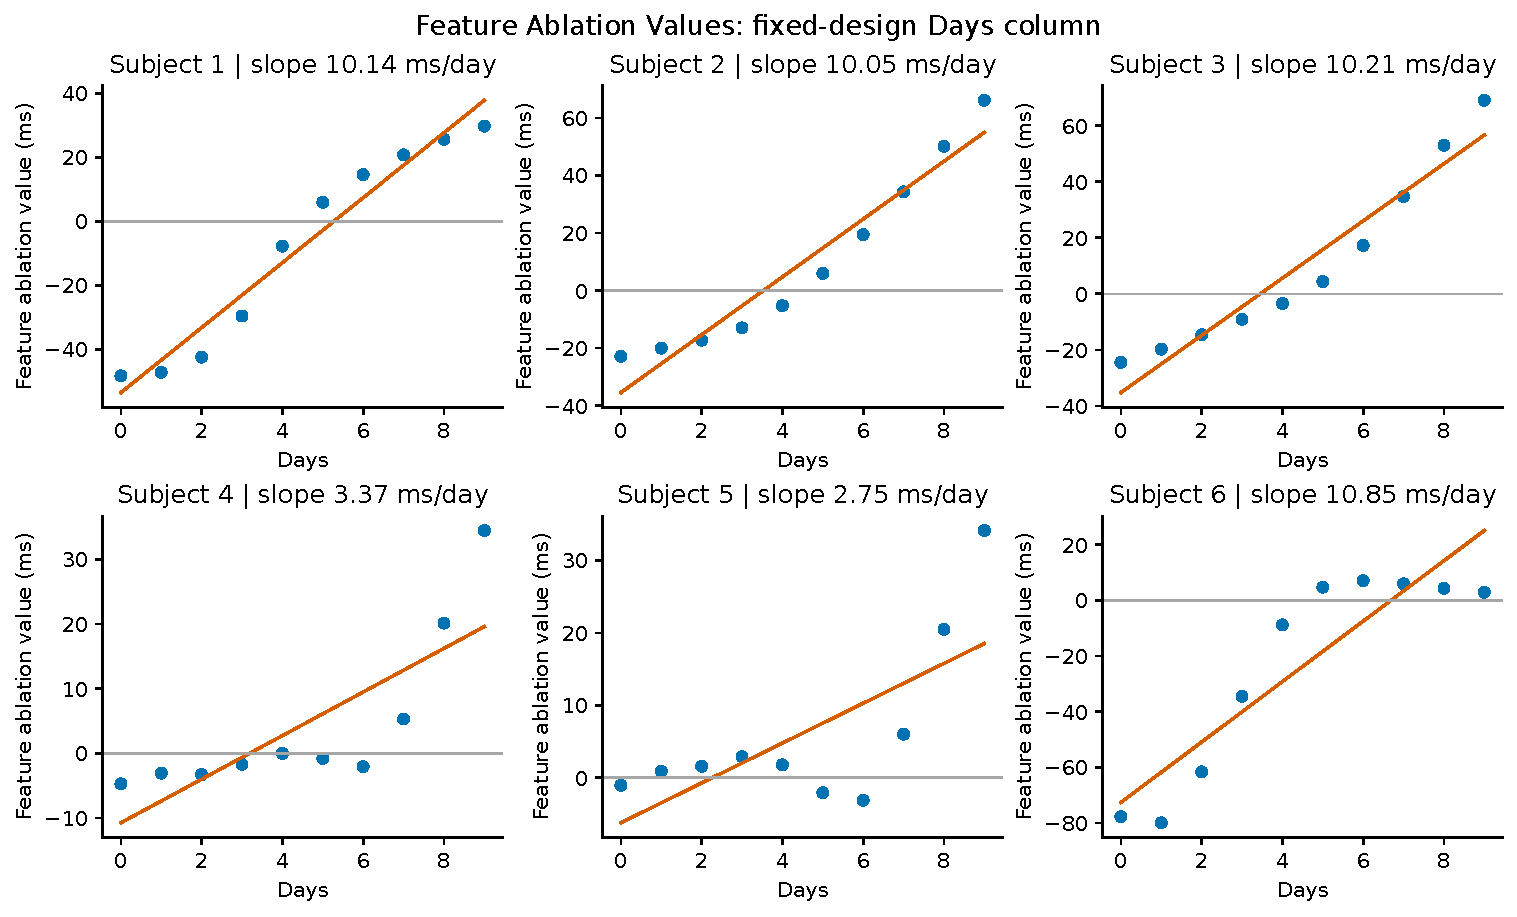
\includegraphics[width=\textwidth]{shap_days_effect_per_subject.pdf}
\caption{Fixed-design Days ablation values for six subjects, in milliseconds. Each point is the prediction minus its value after replacing the fixed-design Days column by the training-background mean, with the random-slope inputs and group indices held fixed. Lines are descriptive least-squares summaries, with slopes in ms/day. This is a full-data illustration, not held-out prediction assessment or recovery of subject-specific random coefficients. Subjects have anonymous source-order labels.}
\label{fig:ablation_days_effects}
\end{figure}

\begin{figure}[htbp]
\centering
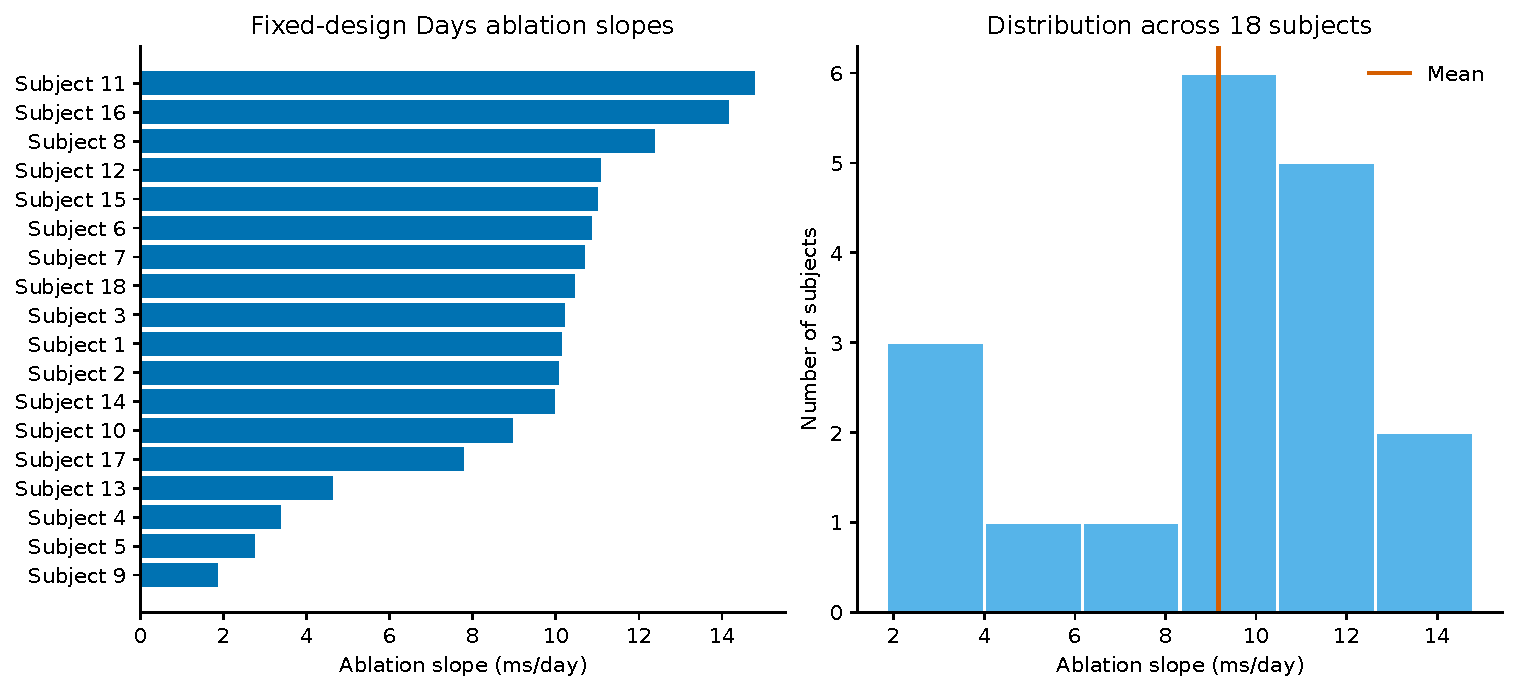
\includegraphics[width=\textwidth]{shap_subject_effect_comparison.pdf}
\caption{Ablation slopes from the fixed-design Days perturbation across all 18 subjects. Left: ordered descriptive line slopes in ms/day. Right: their distribution, with a line marking the mean. These summaries describe the fitted function under a specified perturbation; they do not estimate the random-slope variance component.}
\label{fig:ablation_subject_comparison}
\end{figure}

\begin{figure}[htbp]
\centering
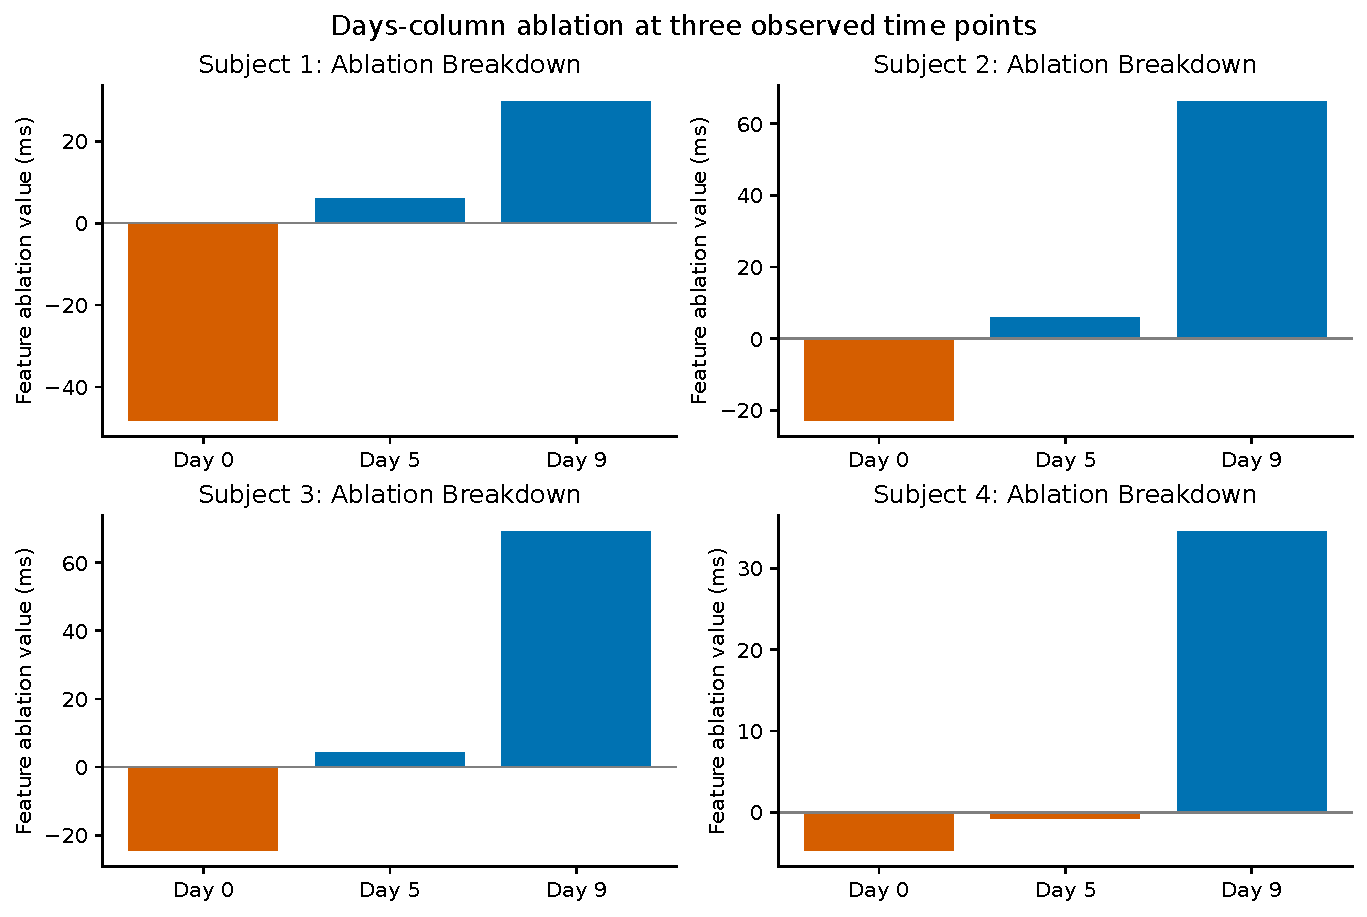
\includegraphics[width=0.95\textwidth]{shap_waterfall_subjects.pdf}
\caption{Ablation breakdown for four subjects at observed Days 0, 5 and 9. Bars show the single fixed-design Days-column prediction difference in milliseconds, using the same background and frozen random-slope inputs as Figure~\ref{fig:ablation_days_effects}. Bars describe separate observations and are not accumulated to reconstruct a prediction.}
\label{fig:ablation_breakdown}
\end{figure}

\FloatBarrier

The fitted lines in Figure~\ref{fig:ablation_days_effects} summarize the plotted perturbations; they are neither random-slope coefficients nor causal effects of sleep deprivation. Figure~\ref{fig:ablation_subject_comparison} summarizes their distribution. Figure~\ref{fig:ablation_breakdown} displays the same column perturbation at three observed days; its bars are not an additive decomposition of a prediction. The complete generator is \texttt{create\_feature\_ablation\_plots.py} in the experiments directory.

\subsection{Scope of the Empirical Evidence}

These experiments evaluate Gaussian regression, binomial classification and one component comparison. They do not evaluate survival prediction, multitask benefit, genomic prediction or the spatial manifold backbone. The repeated splits probe sensitivity to the held-out rows or groups, but limited model configurations leave tuning sensitivity unresolved. Specialized mixed-effects machine-learning baselines such as LMMNN and GPBoost are not evaluated. The package supports these additional interfaces, but no performance claim for them follows from the present results.


\section{Discussion and Conclusion}
\label{sec:discussion}

We have presented TabMixNN, a comprehensive framework for mixed-effects deep learning on tabular data. The framework successfully bridges classical statistical modeling and modern neural networks through:

\begin{itemize}
    \item \textbf{Modular architecture}: Clean separation of encoder, backbone, and output heads enables flexible composition
    \item \textbf{Rich covariance structures}: Support for temporal (AR/ARMA), spatial (GP/SPDE), and genetic (kinship) correlation
    \item \textbf{Diverse outcome families}: Unified interface for regression, classification, and multitask learning
    \item \textbf{Structural regularization}: Ordered triangular blocks and optional sparsity penalties
    \item \textbf{Interpretability}: Parameter extraction, variance decomposition, and single-feature ablation values
    \item \textbf{Accessibility}: R-style formula interface and scikit-learn compatibility
\end{itemize}

\subsection{Limitations and Future Work}

Current limitations and directions for future research include:

\begin{itemize}
    \item \textbf{Scalability}: For very large datasets ($n > 10^6$), additional optimizations (distributed training, approximations) may be needed
    \item \textbf{Automatic structure search}: The present triangular parameterization fixes a channel ordering; it does not search all DAG orderings
    \item \textbf{Uncertainty quantification}: Observation-noise integration, uncertainty in network/covariance parameters and predictive coverage require additional work
    \item \textbf{Non-Euclidean data}: Extensions to graphs, manifolds, and other non-tabular structures
    \item \textbf{Identifiability}: Centering does not identify all latent coordinates, and predictive structural edges do not have a causal interpretation without additional assumptions
    \item \textbf{Evaluation scope}: Five repeated holdouts and three neural seeds describe split and initialization sensitivity but do not estimate independent sampling uncertainty. Small group counts, limited baseline tuning and the absence of external validation limit generalization; survival, multitask and spatial/genomic applications are not benchmarked here
    \item \textbf{Fairness and privacy}: Incorporation of fairness constraints and differential privacy
\end{itemize}

\subsection{Conclusion}

TabMixNN combines variational mixed-effects encoding with neural prediction for grouped tabular data. In the ten-dataset evaluation, five-split mean RMSE and AUROC favor TabMixNN over the fixed neural control on all known-group tasks, although some differences are small. Performance for entirely unseen groups varies by dataset. TabMixNN has lower mean RMSE than XGBoost on three of five unseen-group regression tasks, but the classical mixed model has higher mean AUROC on all five unseen-group classification tasks. The calibration diagnostics also limit the interpretation of fitted probabilities as absolute risks. These results support a task-dependent software contribution; exploratory dataset selection, fixed tuning choices and the absence of external validation limit broader conclusions.

% \section*{Acknowledgments}

% Acknowledgments will be added

\FloatBarrier
\appendix
\section{Linear equivalence, variational gap and identifiability}
\label{app:linear}

\subsection{The fixed-covariance Gaussian special case}
Let $\mathbf y\in\mathbb R^N$, let $\mathbf X$ have full column rank, and consider
$\mathbf y=\mathbf X\boldsymbol\beta+\mathbf A\mathbf v+\boldsymbol\epsilon$,
where $\mathbf A=\mathbf Z\mathbf L$, $\mathbf v\sim\N(\mathbf0,\mathbf I)$,
and $\boldsymbol\epsilon\sim\N(\mathbf0,\sigma_e^2\mathbf I)$ independently.
Here $\mathbf L$ and $\sigma_e^2>0$ are fixed. There is one scalar response,
an identity decoder, no centering and no additional penalty. For
$q(\mathbf v)=\N(\mathbf m,\mathbf D)$ with positive diagonal $\mathbf D$,
the negative ELBO, up to constants, is
\begin{equation}
 \mathcal F=\frac{\|\mathbf y-\mathbf X\boldsymbol\beta-\mathbf A\mathbf m\|^2
             +\operatorname{tr}(\mathbf A^T\mathbf A\mathbf D)}{2\sigma_e^2}
       +\frac12\{\mathbf m^T\mathbf m+\operatorname{tr}\mathbf D-\log|\mathbf D|\}.
\end{equation}
Differentiating in $\boldsymbol\beta$ and $\mathbf m$ gives
\begin{equation}
 \begin{bmatrix}
 \mathbf X^T\mathbf X & \mathbf X^T\mathbf A\\
 \mathbf A^T\mathbf X & \mathbf A^T\mathbf A+\sigma_e^2\mathbf I
 \end{bmatrix}
 \begin{bmatrix}\widehat{\boldsymbol\beta}\\\widehat{\mathbf m}\end{bmatrix}
 =\begin{bmatrix}\mathbf X^T\mathbf y\\\mathbf A^T\mathbf y\end{bmatrix}.
\end{equation}
These are the Gaussian mixed-model normal equations in innovation coordinates.
The positive prior precision and full-rank fixed design make this mean problem
strictly convex. Thus the optimum mean agrees with generalized least squares
and the conditional random-effect mean at the specified covariance parameters.
This statement concerns the optimum, not a guarantee that a finite stochastic
training run attains it.

\subsection{Why matching the mean does not establish ML or REML equivalence}
For fixed $\boldsymbol\beta$, define
$\mathbf P=\mathbf I+\mathbf A^T\mathbf A/\sigma_e^2$ and
$\mathbf h=\mathbf A^T(\mathbf y-\mathbf X\boldsymbol\beta)/\sigma_e^2$.
The exact conditional posterior is
$\N(\mathbf P^{-1}\mathbf h,\mathbf P^{-1})$.
The diagonal variational optimum has the same mean but
\begin{equation}
 D_{jj}=P_{jj}^{-1},\qquad
 \min_q\operatorname{KL}\{q\|p(\mathbf v\mid\mathbf y,\boldsymbol\beta)\}
 =\frac12\log\frac{\prod_j P_{jj}}{|\mathbf P|}.
\end{equation}
The variance identity follows by differentiating
$\tfrac12\sum_j(P_{jj}D_{jj}-\log D_{jj})$.
Substitution into the Gaussian KL gives the displayed gap. It is nonnegative
by the determinant inequality for positive definite matrices and vanishes
when $\mathbf P$ is diagonal. The gap depends on covariance parameters through
$\mathbf P$. Optimizing a diagonal ELBO over those parameters therefore need
not optimize the marginal likelihood. REML additionally accounts for fixed-effect
estimation and is not implemented by this objective.

For example, with
\begin{equation}
 \mathbf P=\begin{bmatrix}2&1\\1&2\end{bmatrix},\quad
 \mathbf P^{-1}=\frac13\begin{bmatrix}2&-1\\-1&2\end{bmatrix},\quad
 \mathbf D=\frac12\mathbf I,
\end{equation}
the gap is $\tfrac12\log(4/3)$. Each variational marginal variance is $1/2$
instead of $2/3$. Nevertheless, the variance of $v_1+v_2$ is $1$ under $q$
and $2/3$ under the exact posterior, whereas for $v_1-v_2$ the corresponding
variances are $1$ and $2$. Predictive uncertainty can therefore be distorted
in either direction. The distinction between mean accuracy and covariance
accuracy is also emphasized by \citet{giordano2018covariances}.

\subsection{A scale invariance in the neural encoder}
\label{app:scale}
Consider an uncentered IID encoder with representation
$\mathbf H=\mathbf X\mathbf W+\mathbf Z\mathbf L\mathbf v$ and a downstream
learned projection $\mathbf H\mathbf C+\mathbf b$. For any $c>0$, replacing
$(\mathbf W,\mathbf L,\mathbf C)$ by
$(c\mathbf W,c\mathbf L,\mathbf C/c)$ leaves every downstream prediction
unchanged, for every latent draw. Keeping $q(\mathbf v)$ fixed also preserves
the innovation-space KL. In the absence of scale-breaking penalties this
preserves the ELBO while changing the encoder prior covariance from
$\mathbf L\mathbf L^T$ to $c^2\mathbf L\mathbf L^T$.
The implementation test uses $c=3$ in a nonlinear network and checks both
predictions and objective values. Thus encoder covariance magnitudes are not
uniquely identified response-scale variance components. Centering alone does
not resolve this scale invariance. An identity decoder fixes this particular
rescaling, but does not establish general identifiability for neural models.

\subsection{Verification coverage}
The Gaussian normal-equation test checks gradients at an independently solved
mixed-model optimum. A separate symbolic script verifies the two-dimensional
mean and variance derivatives and the exact covariance counterexample.
End-to-end synthetic tests cover fit, prediction, row batching and persistence
for all ten families; survival tests compare likelihoods and predictions with
closed forms. These checks establish specified mathematical and software
contracts. They are not evidence of real-data survival performance, calibrated
prediction intervals, causal identification or global optimization.

\FloatBarrier
\bibliographystyle{plainnat}
\bibliography{references}

\end{document}
